\subsection{Критерий непрерывности монотонной функции.}

\textbf{Теорема.} Пусть $f(x)$ монотонна (например, возрастает $f(x) \uparrow$) на промежутке $\langle a, b \rangle$. Тогда:
\[ f(x) \in C\langle a, b \rangle \iff f(\langle a, b \rangle) \text{ — промежуток (без «дырок»)} \]

\begin{tcolorbox}[title=Доказательство]
    \textbf{1. Необходимость ($\Rightarrow$)}
    Дано: $f(x)$ непрерывна на $\langle a, b \rangle$.
    Из \textbf{теоремы о промежуточном значении} следует, что образ промежутка при непрерывном отображении есть промежуток. (В этом пункте монотонность не используется, только непрерывность).
    
    \textbf{2. Достаточность ($\Leftarrow$)}
    Доказываем от противного.
    Пусть $f(\langle a, b \rangle)$ — промежуток, но $f(x) \notin C\langle a, b \rangle$ (функция разрывна).
    
    Тогда существует точка разрыва $x_0 \in \langle a, b \rangle$.
    
    \textbf{а) Пусть $x_0 \in (a, b)$ (внутренняя точка).}
    Так как $f(x)$ монотонна, существуют односторонние пределы:
    \[ \lim_{x \to x_0 - 0} f(x) \quad \text{и} \quad \lim_{x \to x_0 + 0} f(x) \]
    В силу возрастания ($f(x) \uparrow$):
    \[ \lim_{x \to x_0 - 0} f(x) \le f(x_0) \le \lim_{x \to x_0 + 0} f(x) \]
    
    Так как $x_0$ — точка разрыва, эти пределы не могут быть равны. (Если бы они были равны, то они равнялись бы и $f(x_0)$, и функция была бы непрерывна).
    Следовательно:
    \[ \lim_{x \to x_0 - 0} f(x) < \lim_{x \to x_0 + 0} f(x) \]
    
    Это означает, что существует "разрыв" (скачок) в значениях функции.
    Возьмем любое число $A$ из интервала между пределами:
    \[ \exists A \in \left( \lim_{x \to x_0 - 0} f(x), \; \lim_{x \to x_0 + 0} f(x) \right), \quad A \neq f(x_0) \]
    
    Так как функция возрастает, она не может принять значение $A$ ни слева от $x_0$ (там значения меньше левого предела), ни справа от $x_0$ (там значения больше правого предела), ни в самой точке $x_0$ (так как $A \neq f(x_0)$).
    
    \textbf{Вывод:} Значение $A$ не принимается на $\langle a, b \rangle$.
    Значит, множество значений $f(\langle a, b \rangle)$ не содержит точку $A$, хотя содержит точки меньше и больше $A$. Следовательно, образ не является промежутком («дырка»). \textbf{Противоречие.}
    
    \textbf{б) Пусть $x_0 = a$ или $x_0 = b$ (граничные точки).}
    Рассуждение аналогично. Если в граничной точке разрыв, то возникает интервал значений между $f(a)$ и пределом $\lim_{x \to a+0} f(x)$, которые функция не принимает. Образ снова не является промежутком.
    
    \begin{center}
    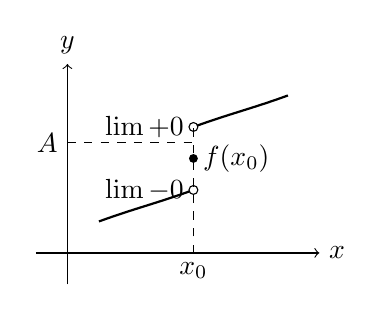
\begin{tikzpicture}[scale=0.8]
        % Оси
        \draw[->] (-0.5,0) -- (4,0) node[right] {$x$};
        \draw[->] (0,-0.5) -- (0,3) node[above] {$y$};
        
        % Разрыв
        \draw[thick] (0.5, 0.5) to[out=20,in=200] (2, 1);
        \draw[fill=white] (2,1) circle (2pt);
        \node[left] at (2,1) {$\lim -0$};
        
        \draw[thick] (2, 2) to[out=20,in=200] (3.5, 2.5);
        \draw[fill=white] (2,2) circle (2pt);
        \node[left] at (2,2) {$\lim +0$};
        
        % Значение в точке
        \fill (2, 1.5) circle (2pt) node[right] {$f(x_0)$};
        
        % Проекция
        \draw[dashed] (2,0) node[below] {$x_0$} -- (2, 2);
        
        % Дырка в значениях (A)
        \draw[dashed] (0, 1.75) node[left] {$A$} -- (2, 1.75);
    \end{tikzpicture}
    \end{center}
\end{tcolorbox}
